% called by main.tex
%
\chapter{Resultados y análisis}
\label{ch::resultados}

Este capítulo separa dos niveles de evidencia que no deben confundirse. Primero se presenta
la evaluación confirmatoria del especialista base, congelado antes de observar el bloque del
6 al 10 de junio. Después se documenta el diagnóstico de volatilidad realizado sobre ese mismo
bloque. El segundo resultado es útil para formular una política futura, pero no constituye
una nueva validación fuera de muestra.

\section{Resultados obtenidos}

\subsection{Validación fuera de muestra del especialista base}

El especialista congelado selecciona 754 unidades de acción en los cinco días fuera de
muestra. Sin aplicar ningún filtro decidido a partir de esos datos, obtiene un neto medio de
$+0{,}349$ ticks al coste de referencia. El promedio es positivo en tres de cinco días y
pasa a ser ligeramente negativo ($-0{,}026$ ticks) cuando se carga el coste visible completo
(Tabla~\ref{tab:fresh}). Esta es la estimación limpia del rendimiento fuera de muestra.

\begin{table}[h]
\centering
\caption{Validación fuera de muestra del especialista base congelado. Los valores son ticks
netos por unidad de acción y no incorporan el filtro de volatilidad posterior.}
\label{tab:fresh}
\begin{tabular}{lr}
\toprule
\textbf{Métrica} & \textbf{Valor} \\
\midrule
Unidades de acción ($n$)                  & 754 \\
Días de soporte                          & 5 (3/5 positivos) \\
Neto medio (coste 0,25, optimista)         & $+0{,}537$ ticks \\
Neto medio (coste 0,5, referencia)         & $+0{,}349$ ticks \\
Neto medio (coste 1,0, estrés)             & $-0{,}026$ ticks \\
\bottomrule
\end{tabular}
\end{table}

\begin{table}[h]
\centering
\caption{Desglose diario del especialista base al coste de referencia.}
\label{tab:base_daily}
\begin{tabular}{lrr}
\toprule
\textbf{Día} & \textbf{$n$} & \textbf{Neto medio @0,5} \\
\midrule
6 de junio  & 220 & $+0{,}666$ \\
7 de junio  &  97 & $+1{,}342$ \\
8 de junio  & 241 & $+0{,}308$ \\
9 de junio  & 146 & $-0{,}565$ \\
10 de junio &  50 & $-0{,}105$ \\
\bottomrule
\end{tabular}
\end{table}

El signo positivo al coste de referencia indica que el especialista conserva una señal
modesta donde los modelos anteriores habían fracasado. Sin embargo, ni la estabilidad diaria
ni el escenario de coste completo permiten calificarlo como una política robusta. La lectura
defendible es, por tanto, \emph{señal parcial fuera de muestra}, no rentabilidad demostrada.

\subsection{Diagnóstico \emph{post-hoc} del régimen de volatilidad}

La inspección del bloque reveló que la fracción de sesiones de alta volatilidad aumentó hasta
aproximadamente el 58\,\%, frente al 18--22\,\% de los periodos históricos
(Figura~\ref{fig:regimen}). Para estudiar ese desplazamiento se dividió la selección con el
umbral 0,6657, percentil 80 de la volatilidad de entrenamiento. El umbral numérico no se
ajustó al bloque nuevo, pero la decisión de usarlo como filtro sí se tomó tras observarlo; por
ello, todo lo que sigue en esta subsección es diagnóstico y exploratorio.

\begin{figure}[h]
\centering
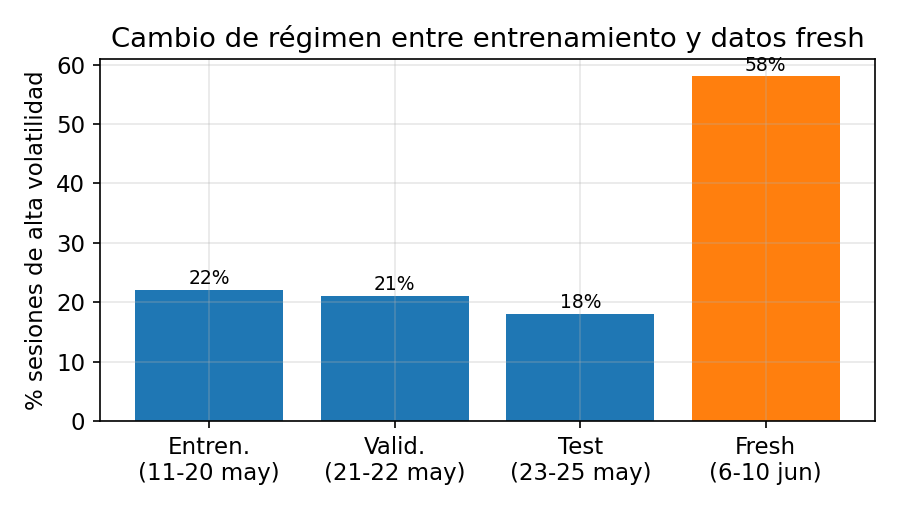
\includegraphics[width=0.6\textwidth]{figures/fig_regimen.png}
\caption{Fracción de sesiones de alta volatilidad por periodo. El salto del bloque nuevo
motiva el análisis de régimen, pero no valida por sí mismo el filtro.}
\label{fig:regimen}
\end{figure}

La Tabla~\ref{tab:regimen} muestra el contraste. Hay 318 acciones de baja volatilidad, 435 de
alta volatilidad y una acción sin dato de volatilidad, que una regla operativa conservadora
rechazaría. Las primeras son positivas y las segundas, negativas al coste de referencia.

\begin{table}[h]
\centering
\caption{Diagnóstico \emph{post-hoc} por régimen en el bloque del 6--10 de junio (ticks por
unidad de acción).}
\label{tab:regimen}
\begin{tabular}{lrrrr}
\toprule
\textbf{Régimen} & \textbf{$n$} & \textbf{@0,25} & \textbf{@0,5} & \textbf{@1,0} \\
\midrule
Baja volatilidad   & 318 & $+1{,}258$ & $+1{,}069$ & $+0{,}691$ \\
Alta volatilidad   & 435 & $+0{,}004$ & $-0{,}183$ & $-0{,}558$ \\
Volatilidad ausente&   1 & $+3{,}327$ & $+3{,}154$ & $+2{,}807$ \\
\midrule
Total sin filtro   & 754 & $+0{,}537$ & $+0{,}349$ & $-0{,}026$ \\
\bottomrule
\end{tabular}
\end{table}

\begin{figure}[h]
\centering
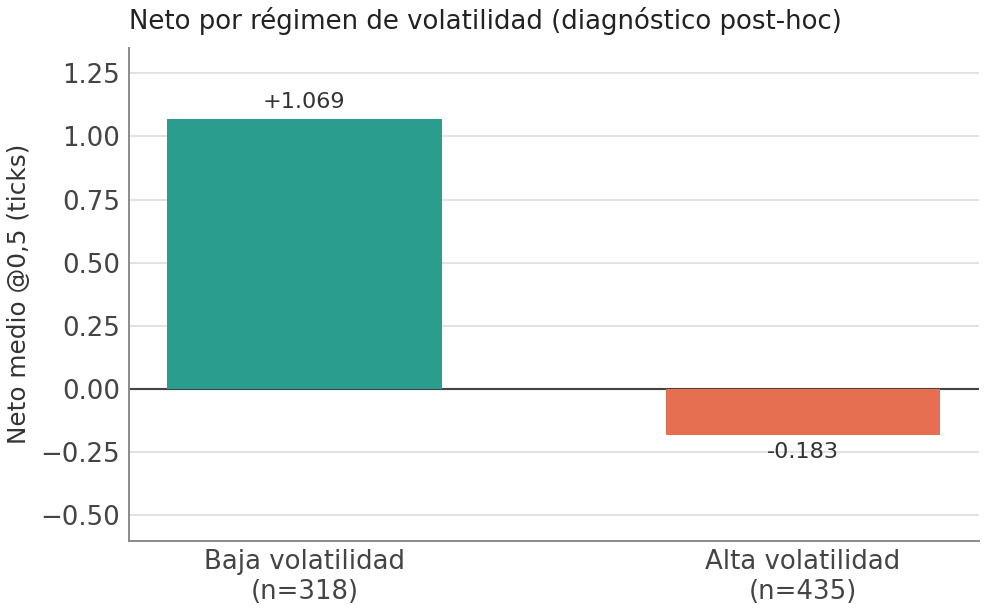
\includegraphics[width=0.56\textwidth]{figures/fig_regimen_neto.png}
\caption{Contraste \emph{post-hoc} del neto medio entre baja y alta volatilidad. La separación
es una hipótesis de política que requiere datos posteriores.}
\label{fig:regimenneto}
\end{figure}

Si se aplica retrospectivamente el filtro de baja volatilidad, el subconjunto de 318 acciones
mantiene signo positivo en los tres niveles de coste (Figura~\ref{fig:coste}) y en los cinco
días (Figura~\ref{fig:netodiario}). Su suma cronológica presenta un drawdown diagnóstico de
88,1 ticks (Figura~\ref{fig:drawdown}). Estas magnitudes describen el subconjunto observado;
no son PnL de una cartera ejecutada.

\begin{figure}[h]
\centering
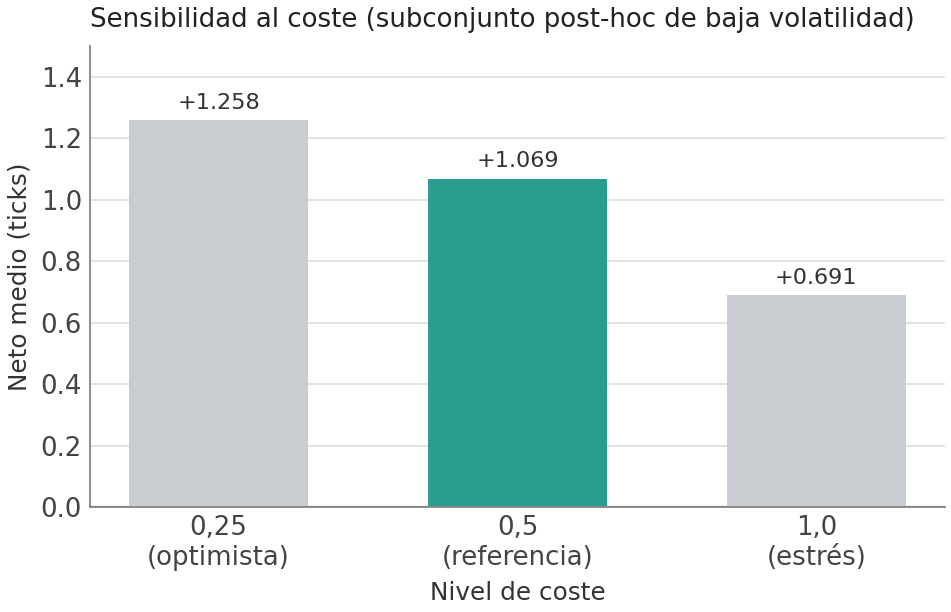
\includegraphics[width=0.55\textwidth]{figures/fig_coste.png}
\caption{Sensibilidad al coste del subconjunto de baja volatilidad. Resultado exploratorio
obtenido tras inspeccionar el mismo bloque.}
\label{fig:coste}
\end{figure}

\begin{figure}[h]
\centering
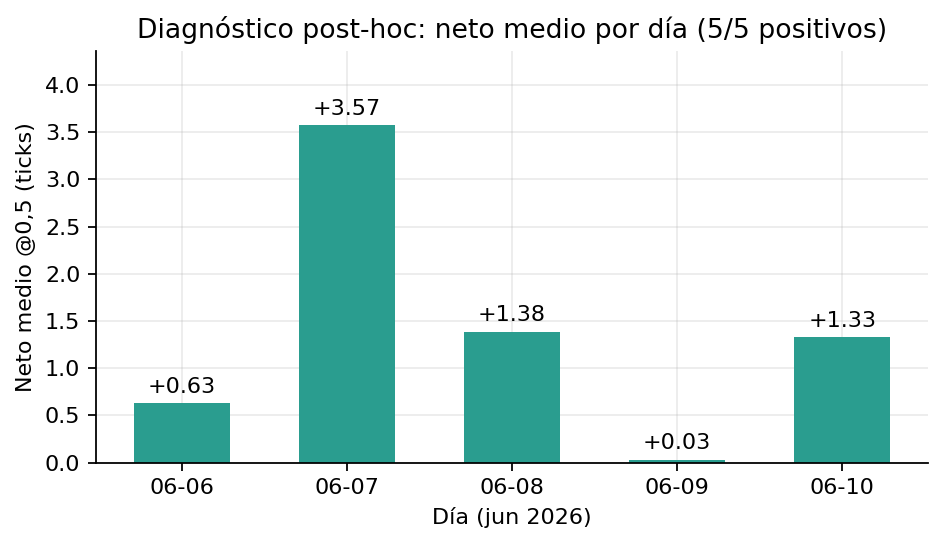
\includegraphics[width=0.62\textwidth]{figures/fig_neto_diario.png}
\caption{Neto medio diario del subconjunto \emph{post-hoc} de baja volatilidad.}
\label{fig:netodiario}
\end{figure}

\begin{figure}[h]
\centering
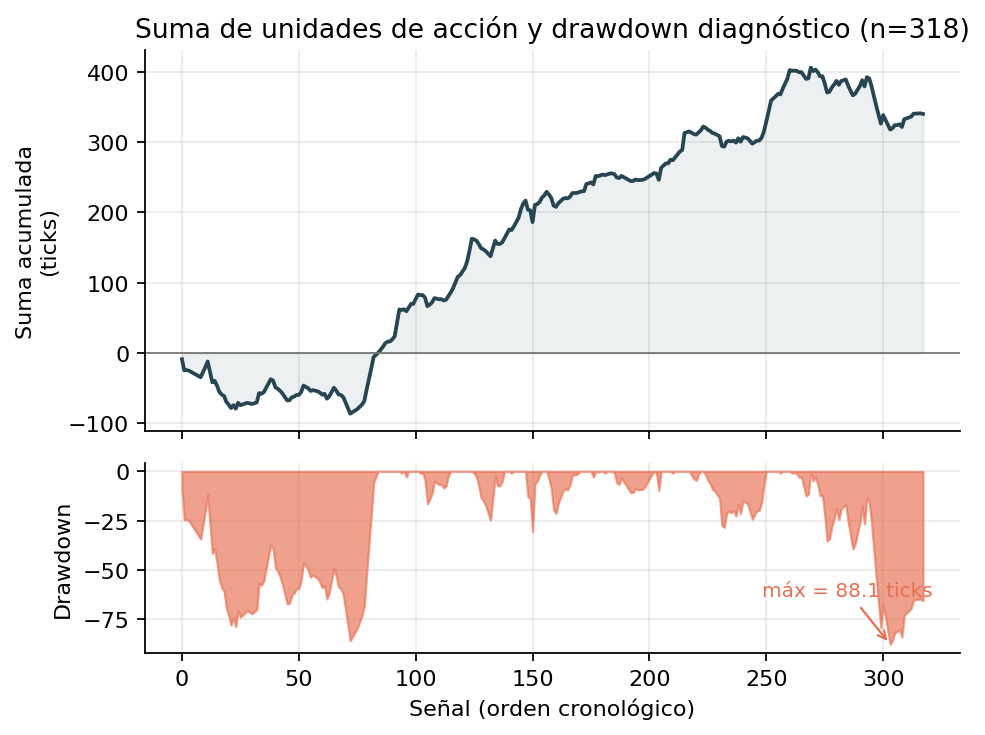
\includegraphics[width=0.62\textwidth]{figures/fig_drawdown.png}
\caption{Suma acumulada y drawdown diagnóstico de 318 unidades de acción. No representa una
cartera con restricciones de capital o de exposición simultánea.}
\label{fig:drawdown}
\end{figure}

El remuestreo independiente de las 318 acciones produce un IC90 de
$[+0{,}472,+1{,}654]$ y $P=0{,}998$, pero esa estimación ignora la dependencia entre señales
del mismo mercado. Hay 156 mercados y hasta ocho acciones por mercado. Un \emph{bootstrap}
agrupado por mercado amplía el IC90 a $[+0{,}193,+2{,}004]$ y reduce la probabilidad estimada
a 97,6~\%. Ambos cálculos son descriptivos: la selección \emph{post-hoc} impide darles una
lectura confirmatoria.

\subsection{Registro de sombra retrospectivo}

Para auditar la mecánica de la política candidata se construyó un registro de sombra
\emph{offline}: conserva cada unidad de acción, su mercado, el resumen diario y las reglas de
promoción. Es una reproducción retrospectiva de lo que la regla habría indicado, no una
ejecución prospectiva ni un sistema activo en tiempo real. El filtro queda congelado después
del 10 de junio; solo observaciones posteriores pueden contar para las puertas de promoción.

Además, varias señales pertenecen al mismo mercado y sus horizontes H60 se solapan. Por ello
se denominan \emph{unidades de acción}, no operaciones independientes, y la suma acumulada no
incorpora una regla de exposición máxima. Una futura sombra prospectiva deberá decidir si
permite apilar posiciones o admite una sola posición por mercado.

\section{Comparativa con otros enfoques y baseline}

Esta sección sitúa el resultado limpio del especialista frente a las alternativas evaluadas:
las arquitecturas profundas sobre el libro de órdenes y los intentos de adaptación al cambio
de régimen. La comparación justifica por qué la mejor señal disponible procede de un modelo
tabular sencillo y no de una red profunda.

\subsection{Especialista tabular frente a aprendizaje profundo}

Las redes recurrentes y convolucionales sobre el libro aprenden representación ---algunas
políticas \emph{proxy} resultan positivas dentro de muestra---, pero esa ventaja no sobrevive
cuando se exige selección causal día a día y estabilidad en todo el bloque de test. Con unas
dos semanas de datos, la capacidad necesaria para generalizar temporalmente excede lo que
las redes pueden estimar de forma fiable.

El modelo tabular con regularización agresiva opera en el extremo opuesto: aumenta su sesgo
pero reduce drásticamente la varianza. Restringir la señal a la ventana \emph{prestart} acota
el espacio de hipótesis. Esa combinación conserva un promedio positivo al coste de referencia
en el bloque intacto, aunque todavía no supera el coste de estrés. El resultado no descarta el
aprendizaje profundo; lo sitúa como una vía a reevaluar cuando el volumen de datos crezca.

\subsection{Experimentos de adaptación al régimen}

Ante el cambio de régimen se probaron reentrenamiento incremental con ventana móvil,
alineación de correlaciones CORAL~\cite{sun2016coral}, un filtro conformal, un
\emph{ensemble} por \emph{bootstrap}, un filtro de volatilidad adaptativo, características
normalizadas por volatilidad y \emph{distillation} de una red convolucional temporal.
Ninguna alternativa produjo evidencia prospectiva robusta con tan pocos días. Este resultado
negativo sigue siendo informativo, pero no permite declarar vencedor al filtro simple sobre
el mismo bloque usado para proponerlo. La comparación definitiva queda aplazada hasta disponer
de nuevos datos bajo una política ya congelada.
